\part{Modelling the afterglow of MMT170817}

%\begin{multicols}{2}
\bf{Note on the physical origin of the afterglow.} As insisted upon in the introduction, MMT170817 is an \it{atypical} event. Nonetheless, the numerous observations of remnants and afterglows of transient electromagnetic events (such as supernovae and gamma ray bursts) indicate a common explanation of afterglows having timescales from days to years, such as that of MMT170817. Matter which is ejected during the previous phases of the phenomenon travels in the local external medium faster than the speed of sound. A shock thus forms at the interface of this shock with the interstellar medium. Interstellar material accumulates at this shock front, is excited and radiates. As the material accumulates, the shock decelerates. The exact nature and origin of the ejected matter, and the characteristics of the medium in which it evolves depends on the specific astrophysical phenomena at hand.

Thus, the models which we will describe here and later confront to observations will concern the radiation of interstellar material which is shocked and radiates through the synchrotron process at the front of a shock formed by the piston effect of ejecta from the merger on the exterior medium, while this shock decelerates as it penetrates the ISM.

\fig{shock}{0.5}{Cut across the shock front, showing the ejected matter, and the interstellar material accumulating a the shock front.}
\section{The physics of afterglows: deceleration dynamics, radiation and astronomical observables}

In this section, we will review the physics which will take part in the modelling of the afterglow of MMT170817. We will successively describe the deceleration of the remnant expanding in the interstellar medium, the radiation of matter at the shock front, and derive the electromagnetic signals which arise from this radiation. The more technical details of these physical processes may be found in \it{Appendix B}.

\subsection{Relativistic deceleration}

We now describe the dynamics of the deceleration of the remnant in the ISM. We will consider for this work two different structures for the ejected matter: a \it{mono-kinetic ejecta}, or a \it{radially stratified ejection}.

We will follow the Lorentz factor $\Gamma(r)$ of the ejected matter once it has reached the exterior radial coordinate $r$.

\bf{Mono-kinetic ejection.} In this case, the matter is ejected with initial energy $E_0$ and a single Lorentz factor $\Gamma_0$. By plowing through the ISM, the shock sweeps up interstellar material and decelerates. By denoting $M_{\rm{ej}}$ the mass of the ejected matter, $m(r)$ the accumulated mass swept up by the shock at radius $r$ from the point of ejection, conservation of energy implies that the initial total energy $\Gamma_0 M_{\rm{ej}} c^2 + m(r) c^2$ is distributed in the ejected mass energy $\Gamma(r) M_{\rm{ej}} c^2$ and the internal energy of the swept up mass $\Gamma(r)^2 m(r) c^2$. Thus:

$$\Gamma(r)^2 m(r) + \Gamma(r) M_{\rm{ej}} = \Gamma_0 M_{\rm{ej}} + m(r) $$

Details on the $\Gamma^2 m c ^2$ form for the thermal energy of the swept-up mass can be found in \it{Appendix B}.


We will consider for our purposes a homogeneous medium with numeric density $n$.

Suppose that the mass $M_{\rm{ej}}$ was ejected into a solid angle $\Omega$ by the central source, for instance in the form of a cone. Then if we neglect any lateral expansion of the ejected matter, the swept us mass at radius will be\footnote{In all generality, we should consider the average mass per particle in the local exterior environment instead of $m_P$.}:

$$m(r)~=~\Omega\int_0^r dr' r' ^ 2 n m_P$$

Thus by introducing the isotropic-equivalent ejected mass $M_{\rm{iso}} = 4\pi M_{\rm{ej}}/ \Omega$, the dimensionless mass parameter $\mu(r) \equiv \frac{m(r)}{M_{\rm{iso}}/\Gamma_0}$, writes:

\[
\begin{array}{lcr}

\mu(r) &= &\frac{\Omega\int_0^r dr' r' ^ 2 n m_P}{M_{\rm{ej}}/\Gamma_0}  \\
 &=& \frac{4\pi r ^ 3}{3 M_{\rm{iso}}/\Gamma_0} n m_P

\end{array}
\]

which no longer depends on the solid angle of ejection.


We may identify the \it{deceleration radius}, $R_{\rm{dec}} = \left( \frac{3 E_0}{4\pi n m_P \Gamma_0^2 c^2}\right) ^ {1/3}$, such that:

$$\mu(r) = \left( \frac{r}{R_{\rm{dec}}} \right)^3 $$

And finally, the solution for $\Gamma(r)$ is easily found to be:

$$\Gamma(r) = \Gamma_0 \frac{-1 + \sqrt{1 + 4\mu(r) + \frac{4\mu(r) ^ 2}{\Gamma_0^2}}}{2 \mu(r)}$$

\bf{Phases of deceleration.}We observe three phases in the deceleration of the shock front:

\begin{enumerate}
	\item For $\mu(r) \ll 1/4$, i.e. $r \ll R_{\rm{dec}}$, in the \it{coasting phase}, no deceleration occurs:

	\cen{$\Gamma(r) \simeq \Gamma_0$}

	\item For $1/4 \ll \mu(r) \ll \Gamma_0 ^ 2$, i.e. $R_{\rm{dec}} \ll r \ll \Gamma_0^{2/3} R_{\rm{dec}} \equiv R_{\rm{N}}$ (\it{newtonian radius}), the front is in a \it{relativistic deceleration phase}, during which the swept-up mass progressively reaches $\Gamma_0 M$:

	\cen{$\Gamma(r) \simeq \frac{\Gamma_0}{\sqrt{\mu(r)}} = \Gamma_0 \left(\frac{r}{R_{\rm{dec}}} \right) ^ {-3/2}$}


	\item For $\Gamma_0^2 \ll \mu(r)$, i.e. $ R_{\rm{N}} \ll r$:

	\cen{$\Gamma(r) \simeq 1$}

	and

	\cen{$\beta(r) \simeq \sqrt{\Gamma_0 (\Gamma_0 - 1)} \left(\frac{r}{R_{\rm{N}}} \right) ^ {-3/2}$}

	This is the \it{Newtonian phase}, and we see that deceleration to non-relativistic velocities requires the sweeping up of a mass on the order of $\Gamma_0 M$.
\end{enumerate}

\bf{Radially stratified structure.} In this case, we suppose that the matter was ejected with an inhomogeneous distribution of velocities: some components were ejected with larger energies than others. We parametrize this distribution giving a cumulative ditribution $E( > \Gamma)$ of energies. It is such that at ejection, the total energy of the matter having a Lorentz factor larger than a given $\hat{\Gamma}$ is $E( > \hat{\Gamma})$.

After the ejection, the higher-velocity component of the ejecta will form the shock front, while the rest of the ejecta lags behind. The front shock decelerating in the ISM, the slower components will catch up to the front shock. This way, the catching-up matter will slow the deceleration down, until the slowest component has caught up. Then, the dynamics are the same as a mono-kinetic ejection starting from the slowest initial velocity.

How to write energy conservation in this case? If the front shock has reached a Lorentz factor $\Gamma$ (at $r$), it means that all the energy which was initially available to the ejected matter with Lorentz factors above $\Gamma$ has already caught-up and been injected into the shock, since we neglect the time it takes for matter to catch-up to the shock. But the energy injected by the shock is that held in internal energy form by the swept-up material at the shock, as in the mono-kinetic ejection case. Thus, we have:

$$ \Gamma(r)^2 m(r) c ^ 2 = E( > \Gamma(r)) + m(r) c ^ 2$$

Notice that this is an implicit equation on $\Gamma(r)$, and that we do not consider here an initial bulk mass which would have a initial energy of $\Gamma_0 M c^2$. Considering an additional bulk mass in this process would simply amount to a discontinueous function $ E( > \Gamma)$.

In the case of a homogeneous medium, this reduces to:

$$\frac{4\pi}{3}r^3 n m_P c^2(\Gamma(r)^2 - 1) = E( > \Gamma) $$


Alternatively, we parametrize the distribution in terms of the \it{relativistic 4-velocity} $u = \Gamma \beta$.

It follows that if the total initial energy is $E_0$ and the largest (resp. smallest) velocity in the ejecta is $u_M$ (resp. $u_m$), then the energy distribution function can be written as:

$$ E( > u) = E_0 g(u) $$,

where $g$ is a function equal to 1 for $u < u_m$, to 0 for $u_M < u$, and decreases between $u_m$ and $u_M$.

The simplest functional form for $g$ which meets these requirements is a power-law with some positive index $\alpha$  containing all the unknown physics of the ejection event. Explicitly, the final deceleration dynamics equation is (note that $\Gamma^2 - 1 = (\Gamma\beta)^2$):

$$\frac{4\pi r^3 n m_P c^2u(r)^2}{3 E_0} = \frac{u(r) ^ {-\alpha} - u_M^{-\alpha}}{u_m ^ {-\alpha} - u_M ^ {-\alpha}} $$

In this case, solving for $\Gamma(r)$ (or equivalently $u(r)$) is not analytical, and we will find $\Gamma(r)$ with help of numerical integration. For our purposes, we fix the value of $\alpha$ to the fiducial value of 5 (\cite{13}). 

\subsection{Synchrotron radiation and self-absorption}

We now turn to the radiation emerging from the shocked matter, which constitutes the afterglow emission.

From now on, we will denote with primes $\p$ the value of quantities measured in the frame of the expanding matter, and without primes those measured in the laboratory (exterior) frame.

\bf{Shock conditions on numeric density and specific internal energy. }What are the conditions at the shock front, where interstellar material is excited and radiates? They are given by the Rankine Hugoniot (e.g \cite{39}) relations. In the case of ultrarelativistic matter (with an adiabatic index of $\gamma = 4/3$), the shock-frame numeric density and internal-to-mass energy ratio are:

$$n\p = (4 \Gamma + 3) n$$

and 

$$\epsilon\p = (\Gamma - 1) $$

\bf{Electron population and magnetic field. }The physical process we consider for radiation is synchrotron radiation. The energy deposited by the shock contributes to the two factors of synchrotron radiation: a magnetic field and a population of relativistic electrons.

The microphysics of the emergence of magnetic fields in astrophysical shocks are unclear (nonetheless, see \it{Appendix E} for a short discussion). From our standpoint, we are concerned only with the strength of the field, and will consider that a free microphysical parameter $\epsilon_B$ relates the field magnitude to the shock-frame energy density, such that:

$$\frac{B\p^2}{8\pi} = \epsilon_B n\p \epsilon\p m_P c^2$$

Likewise, we will consider that the electron population has a simple energy spectrum: it is a power law of index $p$ in the Lorentz factor space as of some minimal Lorentz factor $\Gamma_m$. Note that the energy contained in the electron population is \it{not directional}. On the contrary to the exterior kinetic energy of the shock (emcompassed in $\Gamma(r)$), this electron energy distribution arises from an isotropic momentum distribution in the local frame, and thus may be regarded as internal energy.

We introduce yet another microphysical parameter $\epsilon_e$, which relates the proportion of the local internal energy distribution which is carried by the electrons. By requiring that the electrons carry a fraction $\epsilon_e$ of the total internal energy, we write:

$$\int_{\gamma_m}^\infty d\gamma \mathcal{N}(\gamma)\gamma m_e c^2 = \epsilon_e \epsilon\p m_P c^2$$

Also, normalization of the population density writes:

$$\int_{\gamma_m}^\infty d\gamma \mathcal{N}(\gamma) = 1 $$

With an energy density $\mathcal{N}(\gamma) \propto \gamma^{-p}$, one obtains:

$$\gamma_m= \epsilon_e \frac{m_P}{m_e}\frac{p- 2}{p - 1} (\Gamma - 1)$$


\subsection{Derivation of the astronomical observable: flux density}


\bf{Emission from quasi spherical matter.}

$$D(\theta, t) = \Gamma(t)(1 - \beta(t) \cos(\theta))$$

$$F^{\rm{iso}}(\nu, T) = \frac{1}{4\pi D ^ 2}\int_0^{\infty} dt \int_0^\infty dr \int_0^\pi d\theta\int_0^{2\pi} d\phi r^2 \sin\theta\frac{j\p(\frac{\nu}{D(\theta, t)}, r, t) \delta\left(T - t + \frac{r\cos\theta}{c}\right)}{D(\theta, t)^2} $$
\bf{Emission from a jet seen on axis.}

\[

F^{\rm{on}}(\nu, T, \theta_j) = \left\{
	\begin{array}{lr}
        F^{\rm{iso}}(\nu, T) & \text{if } \Gamma \theta_j \gg 1\\
       	\left(\Gamma \theta_j\right) ^ 2 F^{\rm{iso}}(\nu, T) & \text{if } \Gamma \theta_j \ll 1\\
    \end{array}

\]



\bf{Emission from a jet seen off axis.}

$$ F^{\rm{off}}(\nu, T, \theta_j, \theta_{\rm{obs}}) = a ^ 3 F^{\rm{on}}(\frac{\nu}{a}, aT, \theta_j)$$

$$a = \frac{1 - \beta(t)}{1 - \beta(t) \cos(\theta_{\rm{obs}})}$$

\bf{Final parametrization. }In conclusion, the overall parameters necessary to predict afterglow light curves are:

\begin{itemize}
	\item For the external medium: $n$ and $\epsilon_B$,
	\item For a quasi-spherical remnant: $E_0$ and $\Gamma_0$ in the case of a mono-kinetic ejection, or $E_0$, $u_m$ and $u_M$ in the case of a structured ejecta,
	\item For a jetted ejecta: additional geometrical parameters $\theta_j$ and $\theta_{\rm{obs}}$ with respect to a quasi-spherical remnant.

\end{itemize}

\subsection{An illustration of some predicted light curves}
To conclude this section, we will illustrate the models with some predicted light curves. 

\fig{examples}{0.5}{Some light curves as calculated by our model.}

\bf{Why does a light curve peak? } dynamical or spectral regime shifts.

\bf{On the validity of the simplifications used in our study}
In order to evaluate the errors commited on the light curves produced by our simplified calculations (for spherical models as well as jets), some light curves on typical ranges of parameters are compared with those produced by full-fledged simulations, which do perform equal arrival time intergration in general conic geometries. Figure \ref{angular} reports such comparisons.

\fig{angular}{0.5}{Light curves for off-axis jets as calculated with the complete integration and our simplified version. The agreement is surprisingly good, and justifies the usage of the simplified (and fast) calculation for our purposes.}

We observe the agreement to be good on the paramter ranges of interest for our study case, and we conclude that our calculations are sufficient for our purposes. Note that full-fledged calculations, albeit available, would not suite our purposes as they are slow and not fit for parameter space exploration, as we will perform in the next section.

\section{The afterglow of MMT170817: modelling and results}

In this section, we will answer the question: What is the geometry and the dynamical structure of the matter emitting the observed afterglow?

This will lead us to decline various hypothese regarding the deceleration regime of the remnant and its geometry in order to find a coherent description of the phenomena.

\subsection{Choice and reduction of multi-wavelength data}
As described earlier, the afteglow emission was detected in X-ray, radio and visible bands respectively 9, 16 and $\sim$~150~d post-merger (when the kilonova had sufficiently dimmed in the case of the visible band). According to our emission model, the synchrotron injection and cooling frequencies scale as the following, where the model parameters were scaled to near-best-fit values which we will infer on the following paragraphs (and $p = 2.2$):

\bf{Coasting phase:}

$$\nu_m = 10.2~\rm{GHz} \left(\frac{\Gamma_0}{10} \right)^{4} \left(\frac{n}{10^{-3}~\rm{cm}^{-3}} \right)^{1/2} \left(\frac{\epsilon_B}{10^{-3}} \right)^{1/2} \left(\frac{\epsilon_e}{0.1} \right)^{2} \left(\frac{\frac{p - 2}{p - 1}}{0.167} \right)^{2}$$


$$\nu_c = 9.56 \times 10^8~\rm{GHz} \left(\frac{\Gamma_0}{10} \right)^{-4} \left(\frac{n}{10^{-3}~\rm{cm}^{-3}} \right)^{-3/2} \left(\frac{\epsilon_B}{10^{-3}} \right)^{-3/2}  \left(\frac{t_{\rm{obs}}}{10~\rm{d}} \right)^{-2}$$


\bf{Deceleraton phase:}

$$\nu_m = 1.78 \times 10^{-4}~\rm{Hz} \left(\frac{E_0}{10^{51}~\rm{erg}} \right)^{1/2}  \left(\frac{\epsilon_B}{10^{-3}} \right)^{1/2} \left(\frac{\epsilon_e}{0.1} \right)^{2} \left(\frac{\frac{p - 2}{p - 1}}{0.167} \right)^{2} \left(\frac{t_{\rm{obs}}}{100~\rm{d}} \right)^{-3/2} $$


$$\nu_c = 4.38 \times 10^{21}~\rm{GHz} \left(\frac{E_0}{10^{51}~\rm{erg}} \right)^{-1/2} \left(\frac{n}{10^{-3}~\rm{cm}^{-3}} \right)^{-1} \left(\frac{\epsilon_B}{10^{-3}} \right)^{-3/2} \left(\frac{t_{\rm{obs}}}{100~\rm{d}} \right)^{-1/2}$$


\bf{Newtonian phase:}

$$\nu_m = 1.46 \times 10^{-10}~\rm{Hz} \left(\frac{E_0}{10^{51}~\rm{erg}} \right)^{} \left(\frac{n}{10^{-3}~\rm{cm}^{-3}} \right)^{-1/2} \left(\frac{\epsilon_B}{10^{-3}} \right)^{1/2} \left(\frac{\epsilon_e}{0.1} \right)^{2} \left(\frac{\frac{p - 2}{p - 1}}{0.167} \right)^{2} \left(\frac{t_{\rm{obs}}}{10^5~\rm{d}} \right)^{-1/2} $$

$$\nu_c = 1.11 \times 10^{40}~\rm{GHz} \left(\frac{E_0}{10^{51}~\rm{erg}} \right)^{-3/5} \left(\frac{n}{10^{-3}~\rm{cm}^{-3}} \right)^{-9/10} \left(\frac{\epsilon_B}{10^{-3}} \right)^{-3/2} \left(\frac{t_{\rm{obs}}}{10^5~\rm{d}} \right)^{-1/5} $$


Taking the frequencies reported in table \ref{freqs}, we observe that in our case, all of the frequencies of interest are within the same range of the synchrotron spectrum. Namely, in the conditions of the remnant, we have $\nu_m \ll \nu_{\rm{Radio, R, X}} \ll \nu_c$ at essentially all times.

\begin{table}
\begin{center}
\begin{tabular}{c|c|c}
\bf{Band} & \bf{Central frequency} & \bf{Wavelength}\\
\hline
Radio & 3.0 GHz & 10~cm\\
R & $4.56\times 10^5$~GHz & 657~nm \\
X-ray & $2.42\times 10^8$~GHz & 1.23~nm \\

\end{tabular}
\caption{Frequencies of the EM bands of interest for our study}
\label{freq}
\end{center}
\end{table}

In this domain of the spectrum, the flux scales as $F_\nu \propto \nu^{\frac{1 - p}{2}}$. Thus, using the entire multi-wavelength set of photometry points, one can determine the value of $p$ once and for all, and reduce the set of points to a single band (in our case the 3~GHz band) for the rest of the study. This is done in e.g. \cite{5}, and a value of $p = 2.22\pm0.1$ is found. 

For now on, we will take $p = 2.2$, and use the radio 3~GHz points reported in table \ref{radio}. Also, we will fix the value of $\epsilon_e$ to the fiducial value of 0.1 (see e.g. \cite{41})

\begin{table}
\begin{center}
\begin{tabular}{c|c|c}
\bf{Time (days)} & \bf{Flux ($\mu$Jy)} & \bf{Reference}\\
\hline
16.42 & 18.7\pm6.3 & \cite{12}\\
17.39 & 15.1\pm3.9 & --\\
18.33 & 14.5\pm3.7 & --\\
22.36 & 22.5\pm3.4 & --\\
24.26 &  25.6\pm2.9 & --\\
31.22 & 34.0\pm3.6 & \cite{5}\\
46.26 & 44.0\pm4 & --\\
54.27 &  48.\pm6 & --\\
57.22 & 61.0\pm9 & --\\
93.13 & 70.0\pm5.7 & --\\
115.05 & 89.05\pm20 & --\\
162.89 & 98.0\pm22.5 & --\\
196.79 & 78.9\pm9 & \cite{10}\\
216.91 & 68.\pm21 & \cite{17}\\
256.76 & 55.\pm12 & -- \\


\end{tabular}
\caption{3~GHz fluxes considered for our study.}
\label{radio}
\end{center}
\end{table}

\subsection{Can the afterglow come from a post-GRB relativistic jet?}
The first appoach to solving the origin of the afterglow stems from the standard understanding of GRBs. According to this standard model (see e.g. \cite{27}, \cite{26} sec. 5, \cite{28}), sGRBs are produced by the dissipation of the kinetic energy of a relativistic jet into radiation by processes which are still to elucidate. As described above, the later formation of a shock front by the jet and the plowing of interstellar material decelerates the jet and leads to the decollimation of the radiation emanating from the shocked material. If the decollimation and the emitted flux are such that an exterior observer enters the emission cone, than an afterglow from the relativistic jet is observed. Can this description explain the afterglow of MMT170817?


We calculate light curves produced in such a manner by a mono-kinetic jet of aperture $\theta_j$, initial kinetic energy $E_j$\footnote{Notice that in this vision, the kinetic energy of the jet is the remainder of the jet's kinetic energy after dissipation in gamma radiation.} and uniform Lorentz factor $\Gamma_0$, penetrating an exterior medium of number density $n$ and magnetic microphysical parameter $\epsilon_B$, and observed from a angle of $\theta_{\rm{obs}}$.

\fig{jetbest}{0.5}{Best-fit light curve for the mono-kinetic jet afterglow model, and the monokinetic spherical shell model. None are an acceptable fit.}

Figure \ref{jetbest} illustrates the monokinetic jet best-fit light curve to the radio points, obtained with a reduced $\chi^2$ of 119/9~$\sim$~13. 

We observe that the characteristic $F(\nu, T) \propto T^3$ increase of jet afterglows does not fit the rather slow $F(\nu, T) \propto T^{0.79\pm015}$ (cf. infra) of the radio light curve. Furthermore, the smoothness of the jet afterglow peak constrasts with the strongly localized peak of the radio observations.

We may thus conclude that an acceptable fit to the radio data may not be found in the context of an afterglow produced by a jet-like outflow.


\subsection{A quasi-spherical remnant}

The jetted geometry for the afterglow emitter being ruled out, we now turn to the possibility that the shock front has a quasi-spherical geometry. In this case, the outflow of matter is almost spherical, and the corresponding shock front is a shell.

\bf{A mono-kinetic quasi-spherical remnant. }For the same initial energies and Lorent factors, light curves from spherical and jet geometries will differ only after the jet break occurs for the jet model. Moreover, the relative weakness of the GRB hints to a likely small Lorentz factor for at least some of the matter ejected during the phenomena. Thus, we may predict that in our case of likely low Lorentz factor, spherical and jet geometry light curves of the monokinetic model will behave differently as of early times, the jet break occuring shortly for jet geometry cases.

Indeed, by adjusting only four parameters, $n$, $\epsilon_B$, $E_0$ and $\Gamma_0$, a better fit is found for a monokinetic spherical ejecta model, as illustrated in figure \ref{jetbest}. The corresponding reduced $\chi^2$ is 72/11~$\sim$~6.5. Nonetheless, this model also produces a steep increase, and we can conclude that the dynamics at hand in this model are not satisfactory.

\bf{A radially structured quasi-spherical remnant. }We now turn to the radially structured remnant model. Recall this is a spherical outflow, but with components of various initial velocities, resulting in a continuous catching-up of the shock fromed by the fastest matter by slower matter when the shock decelerates. After the whole outflow has caught up to the shock, the dynamics are identical to those of a monokinetic outflow, but starting from the slowest velocity of the outflow.

In this case, the best fit light curve is found to lie close to the radio data, with $\chi^2 = 3.97/10 \sim 0.4$. The corresponding light curve is shown figure \ref{radial}.

\fig{radial}{0.5}{The best-fit light curve for the synchrotron emission model with a radially structured outflow.}

The dynamical regime shift from catching-up to mono-kinetic shell allows for the sharp maximum of the light curve around 160~d post-merger. Remarkelbly, the increasing and the decreasing phase of the radio data are both correctly followed. We conclude that among the three models we have confronted, a radially structured quasi-spherical remnant reproduces the radio data with the most fidelity.


\subsection{Conclusion}

In conclusion, we have shown that in our model of synchrotron emission from shocked interstellar material as the origin of the afterglow of MMT170817, the most likely configuration is that the ejecta forming the shock has a quasi-spherical structure, and was ejected with a total kinetic energy of $\sim~6~\times 10^{50}$~erg, with Lorentz factors in the range $\sim~2-3$, and it is expanding into a medium of number density $\sim~8~\times~10^{-4}$~cm\sp{-3} and a magnetic microphysical parameter of $\sim~1~\times~10^{-3}$. Details on the actual best-fit parameters and their confidence intervals can be found in table \ref{cocoon}.

\section{Discussion around the results from the afterglow modelling}

\subsection{General discussion}

\bf{Degeneracy of parameters and tightness of fit. }Overall, there is an important degeneracy among the parameters of the radially-structured quasi-spherical model, as indicated by the low $\chi^2_{\rm{red}}$ of 0.4. Indeed, the cited best-fit values are indicative of the typical parameter to obtain the radio data, but small deviations from these values still produce acceptable light curves.

This is illustrated by studying the correlations between parameters. For the two external medium parameters $n$ and $\epsilon_B$, the $\chi^2$ map projected on the ($n$, $\epsilon_B$) plane around the best fit values is presented in figure \ref{n_epsilon_B}. The correlation coefficient between the two variables is --0.6. Physically, a model is found tobe as close tothe data than the same model with a higher density and a lower magnetic parameter. This may be understood grossely by noticing that $B \propto \sqrt(\epsilon_B n)$, and thus for a same $\Gamma(r)$ (which depends on $n$), the emission will be equivalent by approximately conserving $\epsilon_B n$.

\begin{table}
\begin{center}
\begin{tabular}{c|c}
\bf{Parameter} & \bf{Best-fit values (1$\sigma$ confidence interval)}\\
\hline
$\bar{n}$ & (8.1\pm1.5) \times 10^{-4} \rm{cm}^{-3} \\
$\bar{\epsilon_B}$ & (8.1\pm1.5) \times 10^{-4}  \\
$\bar{E_0}$ & (5.61\pm0.6) \times 10^{50} \rm{erg} \\
$\bar{u_m}$ & 1.5\pm0.02 \\
$\bar{u_M}$ & 3.19\pm1. \\
\end{tabular}
\end{center}
\caption{Best-fit parameter values for the quasi-spherical shock with radial velocity structure.}
\label{cocoon}
\end{table}

\begin{figure}
\begin{center}
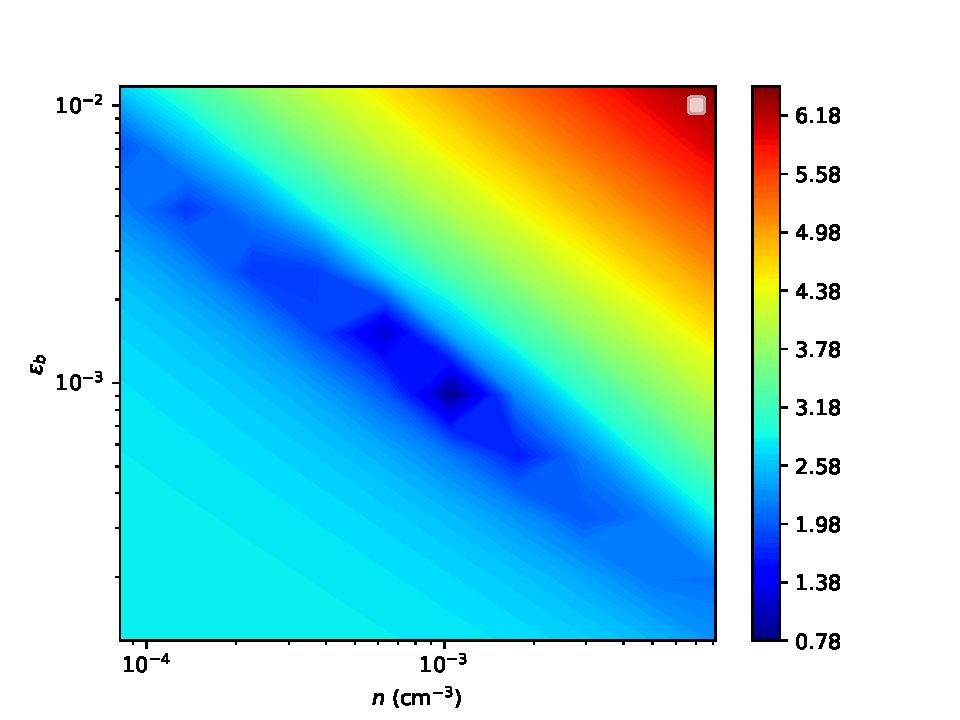
\includegraphics[width=0.5\linewidth]{n_epsilon_B}
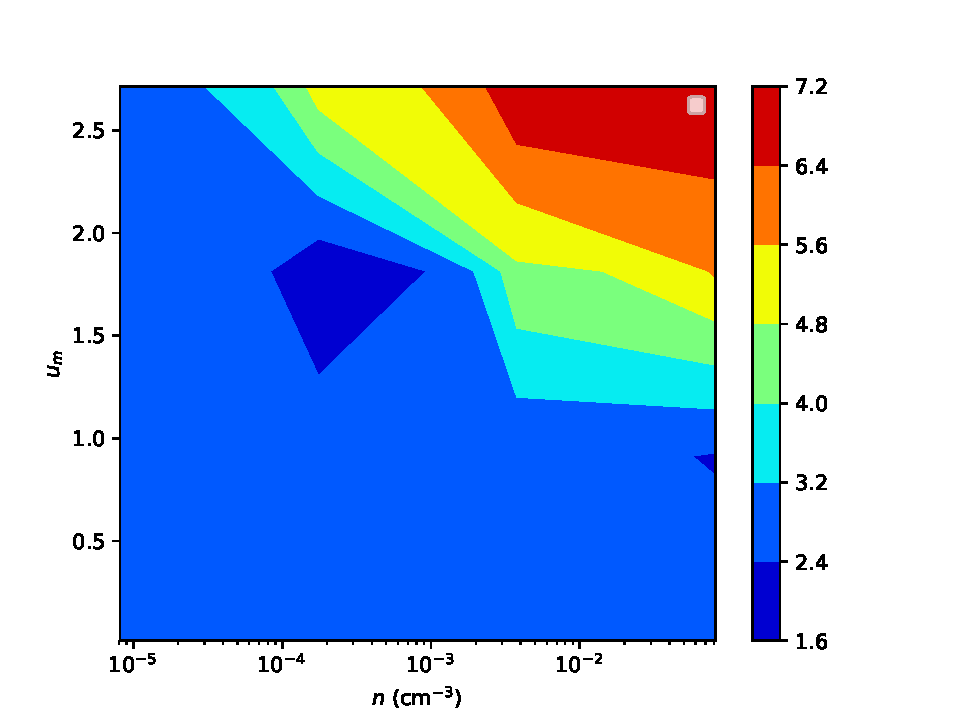
\includegraphics[width=0.5\linewidth]{umn}
\caption{Projected likely-hood map on the fitting of the external parameters $n$ and $\epsilon_B$ (left) and $n$ and $u_m$ (right) in the radially structured ejecta model.}
\label{n_epsilon_B}
\end{center}
\end{figure}


Similarly, we observe a strong anti-correlation between the dynamical parameter $u_m$ and $n$, as shown figure \ref{n_epsilon_B}. We observe that for $u_m$ values smaller than best-fit, the global fitting error is invariant long lines of constant $nu_m^{-\beta}$, where $\beta~\sim~5~=\alpha$. Coming back to the dynamical equation ($V(r) = 4\pi r^3/3$):

$$V(r)c^2 n (u_m^{-\alpha} - u_M^{-\alpha}) = E_0 (u^{-\alpha} - u_M^{-\alpha}) $$

It appears that if $u_m^{-\alpha} \gg u_M^{-\alpha}$, which is the case for our $\alpha = 5$ and $u_m < \bar{u_m} \sim 1.5$, then the dynamic equation simplifies to:

$$V(r)c^2 n u_m^{-\alpha} = E_0 (u^{-\alpha} - u_M^{-\alpha}) $$

by which the dynamics are solely determined by the product $n u_m^{-\alpha}$ as suggested by the anti-correlation we observe.

Also, we deduce from table \ref{cocoon} that the best-constrained parameter is $u_m$. As explained previously, $u_m$ determines the momentwhen the dynamics switch from the catching-up phase to the monokinetic regime, consistently producing a sharp break in the dynamical behavior and thus in the light-curve. As the radio data point out, the flux features a sharp light curve maximum, and it is thus understood that the time of dynamical regime shift must be well determined and thus $u_m$ tightly constrained. 

\bf{What \it{is} the ejected matter? }As we have seen, the aterglow does not likely originate from a post-GRB relativistic jet. It is more likely in a quasi-spherical shape, and was ejected with inhomogeneous velocities. This unfortunately does not inform us on the nature of this ejected matter, i.e. its composition, the process during which, when and from where it was ejected.

It may have been ejected by the friction of the two neutron stars upon coalescence, and later have formed an accretion disk around the final central object and finally been blown away by a thermal neutrino wind, producing the kilonova radiation in the process. It may also be have been emitted by an intermediate central compact object during its relaxation to its final structure as a black hole or neutron star. 

It is likely that the answers to these interrogations lie in the signatures of earlier phases of the phenomenon, such as the kilonova. In particular, as illustrated in figure \ref{gbmax} and table \ref{cocoon}, the maximum ejection velocity $u_M$ is the most poorly constrained parameter of the radially-structured quasi-spherical model, for lack of early radio points. 

\fig{gbmax}{0.5}{Radially structured model light curves with varying $u_M$ and best-fit values for all other paramters. $u_M$ would be better constrained with earlier flux measurements.}


Measuring radio fluxes at earlier times would allow better constraints on $u_M$ and thus a better understanding of the ejection conditions, and therefore of the nature of the ejected matter.

Furthermore, it is possible that the matter currently plowing the exterior medium was not ejected simultaneously. Indeed, in the so-called \it{cocoon model} (\cite{42, 5}, ), a relativistic jet impacts some previously ejected matter, depositing supplementary kinetic energy, and thereby \it{choking} the GRB. This results in no classical jet-produced GRB, but rather in a higher-energy quasi-spherical ejecta producing a weak GRB and eventually a quasi-spherical remnant and shock. Nonetheless, these models concern the origin of the shock-forming matter while our calculations are only concerned with the geometry of this matter and it's final velocity distribution.


\subsection{The external medium}
The best-fit density parameter $\sim~10^{-3}~\rm{cm}^{-3}$ value is broadly consistent with typical values inside gas-rarified early-type galaxies such as NGC4993 (\cite{44}).

More precisely, according to recent measurements of HI 21-cm fluxes in the host galaxy of MMT170817 (\cite{12}), an upper limit on the galaxtic density of atomic hydrogen is found to be $n_{\rm{HI}} < 4 \times 10^{-2}~\rm{cm}^{-3}$. If we suppose (as we have already done in our calculations) that the local medium is composed essentially of hydrogen, this upper limit is consistent with our model's predictions.

Similarly, with a star formation rate measured to $\sim~10\sp{-2}~\Ms/\rm{yr}$ (\cite{9}) and using the Kennicut-Schmidt law  \cite{43}, the average density of HI in NGC4993 is estimated to $\sim~4 \times 10^{-3}~\rm{cm}^{-3}$ (\cite{12}), assuming the HI content to extend out to $\sim~18~\rm{kpc}$ from the center of NGC4993. This is roughly a factor of 2 above our prediction. As illustrated in figure \ref{galac}, the projected position of the coalescence site is well inside the buldge of NGC4993. The angular distance from the merger site to the center of the galaxy is $\sim~10,6''$, equivalent to 2.12~kpc at 40~Mpc.

Consequently, the discrepancy in estimates of local density can be explained either by the fact that the merger site is in fact in a peripheral region of the galaxy, where the density is lower than the average, or on the contrary that the merger site is well inside the galaxy as suggested by the projected position, but the gas and dust content of NGC4993 does not follow an ordinary radially-decreasing profile. This last possibility is further supported by the presence of shell structures in NGC4993 as shown by \cite{33}, indicating a recent galactic merger event implicating the host galaxy, therefore explaining a non-trivial distribution of gas in NGC4993 and finally the possibility for lower-than-average densities even in central regions of the galaxy.

How likely is the merger site to be in the central region of NGC4993? Supposing that the merger site was drawn from a uniform distribution of points in the galaxy of radius $R_G$, the observation of the projected radial distance at $R_\rm{proj} = 2.12$~kpc implies a posterior probability distribution for the actual radial distance $R$ from the galacitc center to the merger locus. This distribution is illustrated in fig \ref{prob}, where we have followed \cite{12} in taking $R_G = 9$~kpc (stellar extent).

\fig{prob}{0.5}{Probability density function for the radial distance of the merger locus to the galactic center, knowing the projected radial distance to be 2.12~kpc, and supposing the merger point drawn at random in the 9~kpc-radius galaxy.}

We observe that the distribution is highly peaked around the projected distance, and nearly uniform in the rest of the density space. It is thus likely that the merger site is really in the center of the galaxy, and if it is not then no further conclusion can be drawn.

\fig{galac}{0.5}{Localisation of the merger site as projected on the sky plane in NGC4993 (\cite{33}).}

\fig{n_vary}{0.5}{Radially structured model light curves with varying exterior density $n$ and best-fit values for other parameters.}




\subsection{What of the standard relativistic jet?}

We found in the previous section that the radio observations could not be understood as the afterglow emission from a jet-structured outflow. Nonetheless, this jet is predicted by standard model of short GRBs. The non-observation of a jet-like afterglow emission therefore constrains the characteristics of any relativistic jet which would have occured and produced the GRB. Furthermore, if we require coherence of these constrained jets with sGRB observations and models, then constrains on the characteristics of the exterior medium are found. 

What can we learn of the eventual relativistic jet from its non-observation until now?

What can we infer on the external medium by confronting these jets with sGRB observations?


\bf{Hiding the jet afterglow.} How may we translate the non-observation of the jet in terms of jet afterglow time of peak and peak flux?

A first approach is to require that the jet-induced afterglow peak flux $F_j^p$ be weaker than the observed radio flux \it{at the time of the jet afterglow peak} $t_j^p$. This of course is a weaker constrain than to require that the jet afterglow flux be \it{weaker than the observed fluxes at all times}. We call this the \it{jet hiding} condition. A mathematical formulation is:

$$F_j^p < F^{\rm{obs}}(\nu, t_j^p) $$

Figure \ref{fmaxtmax} illustrates our method to translate this into conditions in parameter space. Suppose that $F_j^p$ and $t_j^p$ are given in terms of a power-law on the parameters $E_j$, $n$, etc. which we will note $p_1$, $p_2$ for now. That is:

\cen{$F_j^p = F_0 p_1^{\alpha_1} p_2{^\alpha_2} \dots$}

and 

\cen{$t_j^p = t_0 p_1^{\beta_1} p_2^{\beta_2} \dots$}

Then, suppose that the radio light curve be given by a power law as well, that is:

\cen{$\Fobs(\nu, \tobs) = \Fobs_0 \tobs^{\gamma}$}

Now, the hiding condition is thus rewritten:

$$F_0 p_1^{\alpha_1} p_2^{\alpha_2} \dots < \Fobs_0 \left( t_0 p_1^{\beta_1} p_2^{\beta_2} \dots \right)^{\gamma} $$

Which in fact results in a \it{sublinear condition} on the parameters for the jet to be hidden:

$$(\alpha_1 - \gamma \beta_1) \log p_1 + (\alpha_2 - \gamma \beta_2) \log p_2 + \dots < \log \left( \frac{\Fobs t_0 ^\gamma}{F_0} \right) $$

The gemoetrical interpretation of this is simple: the indices $\alpha_i$ and $\beta_i$ are just the coordinates of the vectors by which is dispaced themaximum of the jet afterglow if the parameters are multiplied by 10. The hiding condition is then simply the condition on any linear combination of these vectors so that the jet remain hidden when displacing the maximum, hence changing the underlying parameters.

\fig{fmaxtmax}{0.5}{Illustration of the method used to obtain constraints on the relativistic jet. Changing the jet parameters will displace the maximum of the jet afterglow light curve along the vectors showed here. Requiring that the maximum be always weaker than the radio points amounts to sublinear conditions on the jet parameters.}


After a thorough exploration of the parameter space, we infer that the peak time and peak flux of a jet-induced afterglow consistently scale like the following with the jet parameters and exterior medium parameters\footnote{The initial Lorentz factor of the ejecta $\Gamma_0$ is not relevant here because as detailed in the previous section, the dynamics in the relativistic deceleration phase (during which the peak occurs) no longer depend on $\Gamma_0$}:

$$F_j^p = 121~\mu\rm{Jy} \left(\frac{E_j}{10^{52}~\rm{erg}} \right)^{} \left(\frac{n}{10^{-3}~\rm{cm}^{-3}} \right)^{4/5} \left(\frac{\epsilon_B}{10^{-3}} \right)^{4/5} \left(\frac{\theta_{\rm{obs}}}{0.25~\rm{rd}} \right)^{-4.3} \left(\frac{\theta_j}{0.1~\rm{rd}} \right)^{2} $$

$$t_j^p = 37.4~\rm{d} \left(\frac{E_j}{10^{52}~\rm{erg}} \right)^{1/3} \left(\frac{n}{10^{-3}~\rm{cm}^{-3}} \right)^{-1/3} \left(\frac{\theta_{\rm{obs}}}{0.25~\rm{rd}} \right)^{8/3} $$

We model the observed light curve as a broken power-law as illustrated in figure \ref{fmaxtmax}. We obtain the following:

\[
\Fobs({3~\rm{GHz}}) = \left\{ \begin{array}{lr}
							(77.6 \pm 12.1)~\mu\rm{Jy} \left(\frac{t_{\rm{obs}}}{100~\rm{d}}\right)^{0.791 \pm 0.152} & \text{if}~t_{\rm{obs}} < 163~\rm{d} \\ 
							(45.4 \pm 41.7)~\mu\rm{Jy} \left(\frac{t_{\rm{obs}}}{300~\rm{d}}\right)^{-1.29 \pm 1.56} & \text{if}~163~\rm{d} < t_{\rm{obs}}
							\end{array}\]

In conclusion, a set of jet parameters and exterior medium parameters will give rise to a hidden jet if:

\[ \left\{ \begin{array}{l}
			F_j^p < 77.6 ~\mu\rm{Jy} \left(\frac{t_j^p}{100~\rm{d}}\right)^{0.791} \\
			\rm{and}\\
			F_j^p < 45.4 ~\mu\rm{Jy} \left(\frac{t_j^p}{300~\rm{d}}\right)^{-1.29}
			\end{array}
\]

taking the central values on the power-law fitting of the light curve.

In turn, this translates in parameter space to\footnote{We introduce the notations $\xx{E_j} = \log \left(\frac{E_j}{10^{52}~\rm{erg}} \right)$, $\xx{n} = \log \left(\frac{n}{10^{-3}~\rm{cm}^{-3}} \right)$, $\xx{\epsilon_B} = \log \left(\frac{\epsilon_B}{10^{-3}} \right)$, $\xx{\theta_{\rm{obs}}} = \log \left(\frac{\theta_{\rm{obs}}}{0.25~\rm{rd}} \right)$, $\xx{\theta_j} = \log \left(\frac{\theta_j}{0.1~\rm{rd}} \right)$.}:

\[ \left\{ \begin{array}{l}
			0.736 \xx{E_j} + 1.06\xx{n} + \xx{\epsilon_B} - 5.35\xx{\theta_{\rm{obs}}} + 2\xx{\theta_j} < -0.531\\
			\rm{and}\\
			1.43 \xx{E_j} + 0.37\xx{n} + \xx{\epsilon_B} - 0.49\xx{\theta_{\rm{obs}}} + 2\xx{\theta_j} < 0.74
			\end{array}
\]



These are two sublinear conditions in the 5-dimensional space of jet and medium parameters which are implied by the non-observation of a jet-induced afterglow.

We will now further discuss the eventuality of a relativistic jet and constrain the external medium by specifying some values for some of the parameters in these two sublinear conditions. These values will come either from our previous results (on $n$ and $\epsilon_B$, coming from the fitting to the radially structured remnant light curve), or results from the gravitational wave community (on $\theta_{\rm{obs}}$ mainly) or previous observations and models for GRBs (on $E_j$).



\bf{Further constraints on the external medium.} We will now use these set of conditions to better constrain the external parameters $n$ and $\epsilon_B$.

In order to obtain conditions of $n$ and $\epsilon_B$ only, we must estimate values for $E_j$, $\thetaobs$ and $\theta_j$. Then, the two sublinear constrains which we have derived from the non-pbservation of a jet-like geometry will concern only the exterior medium, through $n$ and $\epsilon_B$.

Which estimate for $E_j$? The fluence of GRB170817A is $(2.08\pm0.2)\times10^{-7}$~erg~cm\sp{-2}, and the isotropic equivalent dissipated energy is $E^{\rm{iso}}_\gamma$~... . In the standard vision where the GRB was produced by a relativistic jet, this is the total kinetic energy of the jet which was dissipated in gamma rays. The kinetic energy of the jet producing the afterglow is thus the remainder of this kinetic energy. By denoting $E^K_0$ the initial kinetic energyof the jet, we thus have:

$$E^K_0 = E^{\rm{iso}}_\gamma + E_j$$

$E_j$ still designating the kinetic energy available for the afterglow if the jet (and which is considered by our model). We now introduce the \it{gamma efficiency} parameter $f_\gamma$, which quantifies the efficiency of the dissipation of kinetic energy into gamma rays in the GRB phase, i.e. $f_\gamma = E^{\rm{iso}}_\gamma/E^K_0$. The efficiencies based on kinetic energy measurements vary from some \% to many tens of \% (\cite{47,48}). Using this definition, it follows that:

$$E_j = \frac{1 - f_\gamma}{f_\gamma} E^{\rm{iso}}_\gamma $$

As for the viewing angle, the gravitational wave data indicates an upper limit $\thetaobs < \thetaobs^{GW} = 28\deg$. We will thus consider various viewing angles below this limit.

For various values of $f_\gamma$, for $\thetaobs = \thetaobs^{GW}$ and $\thetaobs^{GW} / 2$, we plot the exclusion diagram in the $(n, \epsilon_B)$ plane in figure \ref{n_epsilon_B_sup}. We have superimposed the error map from the radially structured model (figure \ref{n_epsilon_B}) for reference.
 
\fig{n_epsilon_B_sup}{0.5}{Superposition of the error map on the fitting of $n$ and $epsilon_B$ to the quasi-spherical radially structured remnant and of the sublinear constraints on these parameters obtained from the hiding of the jet.}

\bf{Discussion on the intrinsic characteristics of the jet.} We now turn to constraining the instrinsic characteristics of the jet. Again, the two sublinear conditions that we have established imply all 5 parameters of a jet afterglow. If we seek constrains on the jet parameters only ($E_j$, $\theta_j$), independently of exterior factors, then we must fix the three parameters $n$, $\epsilon_B$ and $\thetaobs$. Lukily, we have estimates for $n$, $\epsilon_B$ as provided by our fitting to the radially structured model which we can take. Also, we can as above vary $\thetaobs$ in the range indicated by the gravitaional wave data from GW170817.

These constraints in the ($E_j$, $\theta_j$) plane are illustrated in figure \ref{ejthetaj}. The non-shaded region corresponds to possible hidden jets given the likely values of $n$ and $\epsilon_B$ provided by the fitting of the afterglow with a spherical radially structured remnant.

\fig{ejthetaj}{0.5}{Constraints on the intrinsic parameters of the relativistic jet, as visualized in the $(\theta_j, E_j)$ plane for various values of $\theta_{\rm{obs}}$ below $\thetaobs^{\rm{max}} = 28\deg$. }

\fig{angles}{0.5}{Afterglow light curves of jets which respect the constraints imposed by the non-observation}

\bf{Jet-induced bumps.} Of course, our hiding condition on the maximum of the jet afterglow does not fully characterize the non-observation of a jet afterglow. Indeed, if the jet afterglow decays slower than the $t^{-1.3}$ of the radio data, than the jet can create bumps, as illustrated in figure \ref{bump}. Thus, the parameter space which we have excluded here is in fact too loose of a constraint on the jet. In the data of MMT170817 a bump has yet to be found.

\fig{bump}{0.5}{A jet afterglow which complies to our hiding condition (the maximum is weaker than the data at the time of maximum), yet the afterglow is clearly apparent.}

%\end{multicols}